\documentclass[portrait,final,x11names,a1paper,fontscale=0.36]{baposter}

\usepackage{calc}
\usepackage{graphicx,caption}
\usepackage{relsize}
\usepackage{multirow}
\usepackage{rotating}
\usepackage{bm}
\usepackage{url}

\usepackage{graphicx,subfigure}
\usepackage{multicol}

\usepackage{microtype}
\usepackage{helvet}
\renewcommand{\familydefault}{\sfdefault}
\renewcommand{\ttdefault}{lmtt}

% Mathematics
\usepackage{amsmath,amsfonts,amsthm,amssymb,bm}
\usepackage{dutchcal}

\usepackage{numprint}
\npthousandsep{,}\npthousandthpartsep{}\npdecimalsign{.}	

\usepackage{mathtools}
\mathtoolsset{showonlyrefs}

% Valore atteso
\newcommand{\E}[1]{\mathbb{E}(#1)}

% Valore atteso condizionato
\newcommand{\Econd}[2]{\mathbb{E}(#1 \vert #2)}

% Varianza
\DeclareMathOperator{\var}{Var}

% Covarianza
\DeclareMathOperator{\cov}{Cov}

% Correlazione
\newcommand{\corr}[2]{\mathrm{Cor}(#1,#2)}

% Valore assoluto
\newcommand{\abs}[1]{\vert #1 \vert}

% Derivate
\newcommand{\der}[1]{\frac{\partial}{\partial #1}}
\newcommand{\dder}[1]{\frac{\partial^2}{\partial #1^2}}

% Spazio elenchi
\newcommand{\spazio}{\vspace{1.5em}}
\newcommand{\sspazio}{\vspace{3em}}

% Vettore bold
\renewcommand{\vec}[1]{\mathbf{#1}}

\newcommand{\field}[1]{\mathbb{#1}}
\newcommand{\olsbeta}{\hat{\bm{\beta}}_\text{OLS}}

% Math operators
%\DeclareMathOperator*{\argmax}{argmax}
\DeclareMathOperator*{\argmin}{argmin}
\DeclareMathOperator*{\plim}{plim}
\DeclareMathOperator*{\logit}{logit}
\DeclareMathOperator*{\sgn}{sgn}

\newcommand{\widesim}[2][2]{
  \mathrel{\overset{#2}{\scalebox{#1}[1]{$\sim$}}}
  }
  
% Norm
\newcommand{\norm}[1]{\left\lVert#1\right\rVert}

% Rank
\DeclareMathOperator{\rank}{rank}

% Trace
\DeclareMathOperator{\trace}{tr}

% Projection
\DeclareMathOperator*{\proj}{proj_{\perp}}

% Odds
\newcommand{\odds}{\mathrm{Odds}}

% Complementary set
\newcommand{\compl}{\mathsf{c}}

% Function floor
\newcommand{\floor}[1]{\left\lfloor #1 \right\rfloor}

% Function ceiling
\newcommand{\ceil}[1]{\left\lceil #1 \right\rceil}

% Nearest integer function
\newcommand{\nint}[1]{\left\lfloor #1 \right\rceil}

% Indicator function
\usepackage{dsfont}
\newcommand{\indfun}[2]{\mathds{1}_{#1}(#2)}

% Circled numbers
\newcommand*\circled[1]{\tikz[baseline=(char.base)]{
            \node[shape=circle,draw,inner sep=2pt] (char) {#1};}}
     
% Circled numbers (fixed radius)       
\newcommand*\circlef[1]{\tikz[baseline=(char.base)]{
  \draw[fill=white] circle [radius=0.55cm];
  \node[inner sep=2pt] (char) {#1};
}}

% Theorems, definitions, proofs
\newtheorem{theorem}{Theorem}[section]
\newtheorem{proposition}[theorem]{Proposition}
\newtheorem{corollary}{Corollary}[theorem]
\newtheorem{lemma}[theorem]{Lemma}

\newenvironment{definition}[1][Definition]{\begin{trivlist}
\item[\hskip \labelsep {\bfseries #1}]}{\end{trivlist}}

\newenvironment{example}[1][Example]{\begin{trivlist}
\item[\hskip \labelsep {\bfseries #1}]}{\end{trivlist}}

\newenvironment{remark}[1][Remark]{\begin{trivlist}
\item[\hskip \labelsep {\bfseries #1}]}{\end{trivlist}}

\newcommand{\card}[1]{\left\vert #1 \right\vert}

\DeclareMathOperator{\diri}{DP}
\DeclareMathOperator{\ibp}{IBP}
\DeclareMathOperator{\crp}{CRP}


\usepackage[font=small,labelfont=bf,textfont=it]{caption}

\setlength{\columnsep}{1.5em}
\setlength{\columnseprule}{0mm}

\usepackage{enumitem}
\setlist{noitemsep,nolistsep}
\usepackage{stackengine,fontawesome}

\usepackage{tabu}
\usepackage{multicol}
\usepackage{multirow}

\definecolor{blue_icl}{RGB}{0,62,116}
\definecolor{blue_icl2}{RGB}{0,40,255}
\definecolor{navy_icl}{RGB}{0,33,71}
\definecolor{cool_icl}{RGB}{0,110,175}

\newcommand{\icl}[1]{{\bf\color{blue_icl2}{#1}}}

\DeclareMathOperator{\argmax}{argmax}
\usepackage{bm}

\newcommand{\codepath}{./}
\usepackage{minted}
\usemintedstyle{lovelace}
\newcommand{\includeshell}[1] {\inputminted[firstline=1,fontsize=\footnotesize,breaklines]{shell-session}{\codepath/#1}}

% Vettore bold
\renewcommand{\vec}[1]{\boldsymbol{#1}}
\newcommand{\mvec}[1]{\mathbf{#1}}

\usepackage{tcolorbox}
\tcbuselibrary{theorems}
\newtcbtheorem{defi}{Definition}%
{colback=blue_icl2!5,colframe=blue_icl2,fonttitle=\bfseries,left=2pt,right=2pt,top=2pt,bottom=2pt}{th}

% Tables
\usepackage{booktabs}	
\usepackage{array,tabu}
\usepackage{multicol}
\usepackage{multirow}

\begin{document}

\begin{poster}%
  % Poster Options
  {
  % Show grid to help with alignment
  grid=false,
  % Column spacing
  colspacing=1em,
  % Color style
  bgColorOne=white,
  bgColorTwo=white,
  borderColor=blue_icl2,
  headerColorOne=cool_icl,
  headerColorTwo=blue_icl2,
  headerFontColor=white,
  boxColorOne=white,
  boxColorTwo=blue_icl2,
  % Format of textbox
  textborder=roundedleft,
  % Format of text header
  eyecatcher=true,
  headerborder=closed,
  headerheight=0.15\textheight,
  textfont=\bf,
  headershape=roundedright,
  % headershade=shadelr,
  headerfont=\Large\bf,
  textfont={\setlength{\parindent}{1.5em}},
  %boxshade=plain,
  % background=shade-tb,
  % background=plain,
  % bgColorOne=DarkOrange2!40,
  linewidth=2pt,
  columns=5
  }
  % Eye Catcher
  {
\includegraphics[width=14em]{icl_eye.pdf}}%{imperial_logo.pdf}} 
  % Title
  {\centering\color{blue_icl2}{\bf{\huge Automating the selection of  preprocessing  \\[0.1cm]techniques for deep neural networks}}\vspace{0.5em}}
  % Authors
  {\vspace*{-.3cm}
  \hspace*{.8cm} 
  \leavevmode\hbox to \linewidth{ \color{blue_icl2}% 
  \centering
\begin{tabular}[t]{c@{}}
    {\Large{\textbf{Student:} Marcus September}} \\[.05cm]
    {\Large{\textbf{Supervisor:} Francesco Sanna Passino}} \\[.05cm]
\faUniversity\ {Department of Mathematics, Imperial College London} \\
\faEnvelopeO\ {\tt marcus.september22@imperial.ac.uk} \\
%{\large This work is funded by a {\bf Microsoft Security AI} research grant.}
\end{tabular} 
}}

  % University logo
%  {% The makebox allows the title to flow into the logo, this is a hack because of the L shaped logo.
    % \includegraphics[height=9.0em]{images/logo}
%  }

\headerbox{3. Exploratory data analysis}{name=ack,column=0,above=bottom,span=2}{
%\vspace*{.2cm}
 %%%%%%%%%%%%%%%%%%%%%%%%%%%%%%%%%%%%%%%%%%%%%%%%%%%%%%%%%%%%%%%%%%%%%%%%%%%%%%
%\begin{minipage}[t]{0.25\linewidth}
%\hspace*{-0.5cm}
%\includegraphics[width=0.95\textwidth]{1920px-M_box.png}
%\end{minipage} \ \hspace{-0.5cm}
%\begin{minipage}[b]{0.7\linewidth} %\smaller
\noindent
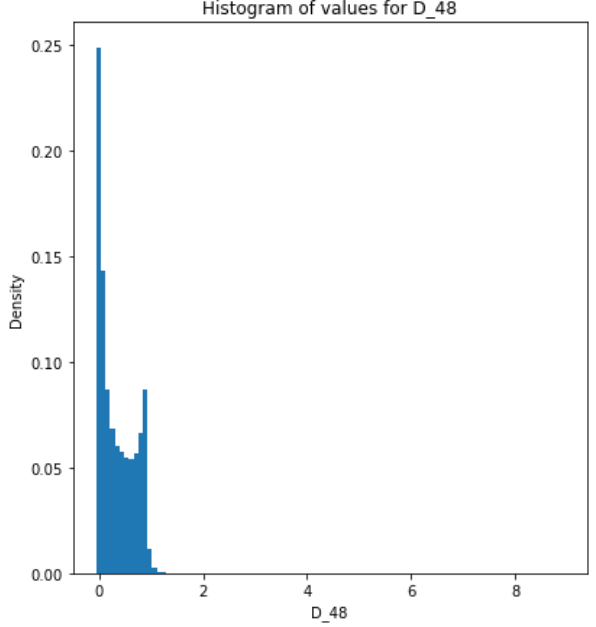
\includegraphics[width=0.48\textwidth]{Figures/eda1.png}
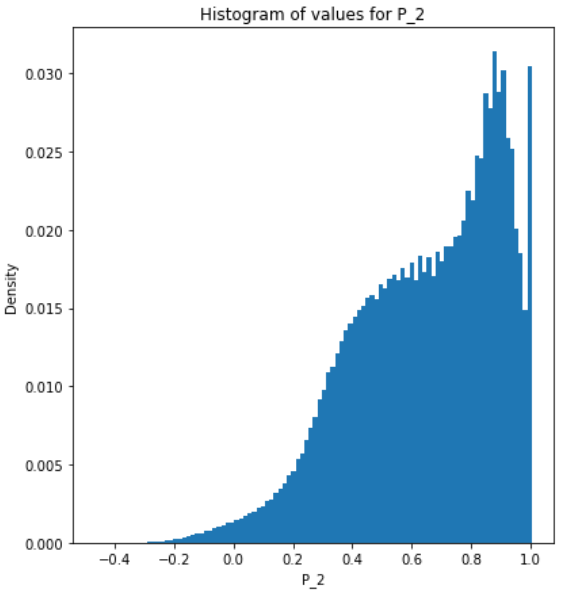
\includegraphics[width=0.48\textwidth]{Figures/eda2.png}
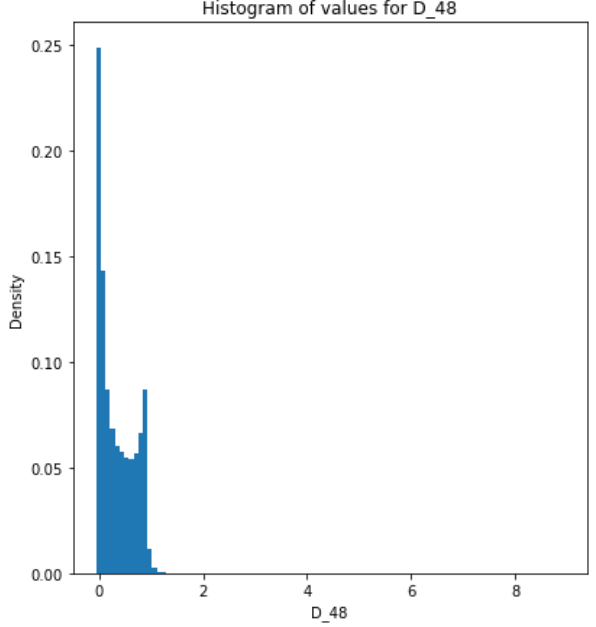
\includegraphics[width=0.48\textwidth]{Figures/eda1.png}
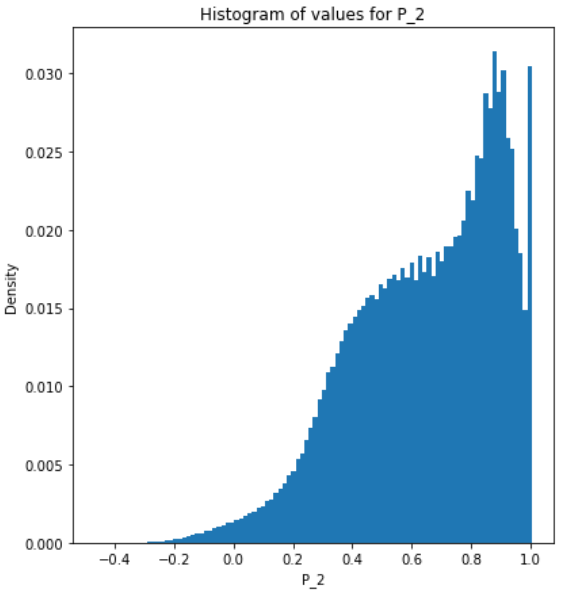
\includegraphics[width=0.48\textwidth]{Figures/eda2.png}

\noindent
A lot of the variables have very skewed distributions or extreme values. There are also many missing values.

%\end{minipage}
%\vspace{.25cm}
%\medskip
}

%%%%%%%%%%%%%%%%%%%%%%%%%%%%%%%%%%%%%%%%%%%%%%%%%%%%%%%%%%%%%%%%%%%%%%%%%%%%%%
  \headerbox{1. Problem and motivation}{name=problem,column=0,row=0,span=2}{
%%%%%%%%%%%%%%%%%%%%%%%%%%%%%%%%%%%%%%%%%%%%%%%%%%%%%%%%%%%%%%%%%%%%%%%%%%%%%%

\noindent   
Deep learning sequence models, such as Recurrent Neural Networks (RNNs) and
transformers, are sensitive to input variable distributions. Both training
speed and performance can drop significantly for non-normal distributions, such
as skewed distributions and those with outliers. Real-world data also usually
contains a lot of missing values, which needs to be converted to numeric values
for use in deep learning models. Deciding on appropriate preprocessing methods
and how to handle missing values is essential in optimising model performance.
However, this is a time-consuming process. The project aims to automate this by
automatically selecting the preprocessing methods to use for any given
sequence dataset, in order to optimise performance and training efficiency.
}


\headerbox{2. Data}{name=data,column=0,row=1,below=problem,above=ack,span=2}{
\noindent
Dataset consists of $N\approx 460000$ customers, each with $P=188$ aggregated
profile features recorded at each of the $T=13$ sequential statement dates.
Together, the dataset forms $N$ instances of a $P$-dimensional multivariate
time-series of length $T$. For each multivariate time-series, the target label
$y \in \{0,1\}$ indicates whether the customer defaulted on their loan or not.
The task is to predict the probability $\mathbb{P}(Y=1)$. Note that due to
privacy concerns, all the dataset features have been anonymized. 
TODO: say something about anonymised with random noise.
}

% \begin{itemize}[leftmargin=.15in]
% \item Consider the \icl{adjacency matrix} $\mvec A=\{A_{ij}\}\in\{0,1\}^{n\times n}$ of a \icl{graph}, where $A_{ij}=1$ if node $i$ connects to node $j$, and $A_{ij}=0$ otherwise. 
% \begin{center}\includegraphics[width=0.75\textwidth]{Pictures/graph.pdf}\end{center}
% \item Graph adjacency matrices can be modelled via \icl{latent position models} (LPMs; Hoff et al., 2002):
% \end{itemize}
% \begin{tabular}{ccccc}
% \parbox{7.5cm}{\centering \vspace*{-0.2cm}{\hspace*{-.75cm}$\vec x_i \overset{iid}{\sim} F\ \rightarrow \mathbb P(A_{ij}=1\vert\vec x_i,\vec x_j)=\kappa(\vec x_i,\vec x_j)\ \rightarrow$}} %\\[0.1cm] $i=1,\dots,n$}} 
% &
% \hspace*{-1.1cm}\raisebox{-.45\height}{\includegraphics[width=.225\textwidth]{Pictures/userdip.png}}
% \end{tabular}
% \begin{itemize}[leftmargin=.15in]
% \item LPMs are built on a powerful idea: expressing \icl{edge-specific probabilities} through \icl{latent node features} $\vec x_i\in\mathcal X\subseteq\mathbb R^d$, using a \icl{kernel function} $\kappa:\mathcal X\times\mathcal X\to[0,1]$. 
%
% \item If the \icl{inner product} is used, the model is known as \icl{random dot product graph} (RDPG; Athreya et al., 2018):
% \begin{equation}
% A_{ij}\vert\vec x_1,\dots,\vec x_n\sim\text{Bernoulli}(\vec x_i^\intercal\vec x_j).
% \end{equation}
% \item RDPGs include many popular network models:
% \begin{itemize}
% \item \icl{Stochastic blockmodels} (SBMs): $\vec x_i=\bm\mu_{z_i}$ for a community $z_i\in\{1,\dots,K\}$, giving a between-community connection probability $B_{k\ell}=\bm\mu_k^\intercal\bm\mu_\ell$;
% \item \icl{Degree-corrected SBMs}: $\vec x_i=\rho_i\bm\mu_{z_i}$ for $z_i\in\{1,\dots,K\}$ and degree-correction $\rho_i\in(0,1)$. 
% \end{itemize}
%
% \item In RPDGs, the latent positions are \icl{estimated via spectral decomposition} of the adjacency matrix. %, with \icl{asymptotic guarantees}. 
% \end{itemize}
%
% \begin{defi}{Adjacency spectral embedding (ASE)}{}
% For an integer $d\in\{1,\ldots,n\}$ and a binary \emph{symmetric} adjacency matrix $\mvec A\in\{0,1\}^{n\times n}$, the $d$-dimensional adjacency spectral embedding %(ASE) 
% $\hat{\mvec X}=[\hat{\vec x}_{1},\dots,\hat{\vec x}_{n}]^\intercal$ of $\mvec A$ is 
% \begin{equation}
% \hat{\mvec X} = \mvec\Gamma\mvec\Lambda^{1/2}\in\mathbb R^{n\times d},
% \end{equation}
% where $\mvec\Lambda$ is a $d\times d$ diagonal matrix containing the absolute values of the $d$ largest eigenvalues in magnitude, %in decreasing order, 
% and $\mvec\Gamma$ is a $n\times d$ matrix containing corresponding %orthonormal 
% eigenvectors.
% \end{defi}
%
% \begin{itemize}[leftmargin=.15in]
% \item For \icl{directed} graphs, the \icl{singular value decomposition (SVD)} is used. 
%
% \item In practice, spectral embeddings often exhibit \icl{manifold structure} (Rubin-Delanchy, 2020).
% \item \icl{Spectral graph clustering} consists in unsupervised detection of groups of nodes from spectral embeddings. 
% \end{itemize}
% \begin{center}
% \includegraphics[width=.95\textwidth]{Pictures/clust.pdf}
% \end{center}
% \begin{itemize}[leftmargin=.15in]
% \item There are two \icl{simultaneous challenges} in graph clustering via spectral embedding under the RDPG: 
% \begin{equation}
% \left.\begin{array}{r}\text{\icl{Manifold}\ structure} \\ \text{\icl{Group}\ structure} \end{array}\right\}\ \text{\icl{Group-specific manifolds}}. 
% \end{equation}
%
% \item \icl{Manifold} structure is accounted for by \icl{latent structure models} (LSM, Athreya et al., 2021): 
% \begin{itemize}
% \item The latent positions $\vec x_i \overset{iid}{\sim} F$ are determined by draws from an underlying univariate distribution $G$ on $[0,1]$, inducing $F$ on a %structural support 
% \icl{univariate submanifold} $\mathcal S\subset\mathbb R^d$. 
%
% \item The distribution $F$ on $\mathcal S$ is the distribution of the %vector-valued 
% transformation $\vec f(\theta)$ of a univariate random variable $\theta\sim G$, where $\vec f:[0,1]\to\mathcal S$ is a function mapping $\theta$ %draws 
% to $\mathcal S$. 
% %\item The inverse function $\vec f^{-1}:\mathcal S\to[0,1]$ could be interpreted as the arc-length parametrisation of $\mathcal S$. 
%
% \item In simple terms, each node is assigned a draw $\theta_i$ from the underlying distribution $G$, representing \textit{how far} along %the submanifold 
% $\mathcal S$ the corresponding latent position lies: %, such that:
% \begin{equation}
% \vec x_i=\vec f(\theta_i).
% \end{equation} 
% %Therefore, conditional on $\vec f$, the latent positions are uniquely determined by $\theta_i$.
% \end{itemize}
% \end{itemize}
% }

%%%%%%%%%%%%%%%%%%%%%%%%%%%%%%%%%%%%%%%%%%%%%%%%%%%%%%%%%%%%%%%%%%%%%%%%%%%%%%
%\headerbox{3. Background: point processes}{name=price,column=1,span=1,row=0}{
  %%%%%%%%%%%%%%%%%%%%%%%%%%%%%%%%%%%%%%%%%%%%%%%%%%%%%%%%%%%%%%%%%%%%%%%%%%%%%%

%\noindent Previous research [1] has demonstrated that mutually exciting processes are suitable for modelling arrival times on a \icl{single edge}. Given arrival times $t_1,t_2,\dots,t_m$ and the corresponding counting process $N(t)=\sum_{i=1}^m \mathds 1_{[0,t]}(t_i)$, the \icl{intensity function} $\lambda(t)$ of a mutually exciting process is:
%\begin{equation}
%\lambda(t) = \lambda + \sum_{k=1+\max\{0,N(t)-r\}}^{N(t)} \omega(t-t_k), 
%\end{equation}
%where $\lambda\in\mathbb R_+$ is a baseline, $\omega(\cdot)$ is an \icl{excitation function}, and $r\in\mathbb N$ is the \icl{number of past events} that contribute to the intensity. 
%Common choices are $r=1$ (Markov process) and $r\to\infty$ (Hawkes process). 
%\fbox{\parbox{.97\textwidth}{\icl{Main issue:} fitting independent processes for each mark $(x,y)$ is computationally expensive, and does not allow to score observations on new edges.}}
%}

%%%%%%%%%%%%%%%%%%%%%%%%%%%%%%%%%%%%%%%%%%%%%%%%%%%%%%%%%%%%%%%%%%%%%%%%%%%%%%
\headerbox{4. Synthetic data}{name=meg,column=2,span=3,row=0, aligned=problem}{
  %%%%%%%%%%%%%%%%%%%%%%%%%%%%%%%%%%%%%%%%%%%%%%%%%%%%%%%%%%%%%%%%%%%%%%%%%%%%%%

\begin{itemize}[leftmargin=.15in]
\item TODO: describe motivation of this and why synthetic data can help
\item TODO
\end{itemize}
}

%%%%%%%%%%%%%%%%%%%%%%%%%%%%%%%%%%%%%%%%%%%%%%%%%%%%%%%%%%%%%%%%%%%%%%%%%%%%%%
\headerbox{5. Evaluation setup}{name=hierarchical,column=2,span=3,row=1, below=meg}{
  %%%%%%%%%%%%%%%%%%%%%%%%%%%%%%%%%%%%%%%%%%%%%%%%%%%%%%%%%%%%%%%%%%%%%%%%%%%%%%

\noindent
\begin{itemize}
    \item TODO: explain cross-validation procedure, and how experimentation framework setup
\end{itemize}
%\item \icl{Full Bayesian model} for LSBM embeddings: 
% \begin{align}
% \hat{\vec x}_i\vert \theta_i,\vec f_{z_i},\bm\sigma^2_{z_i} &\sim \mathbb N_d\left\{\vec f_{z_i}(\theta_i),\bm\sigma^2_{z_i}\mvec I_d\right\},\ i=1,\dots,n,\\
% \theta_i &\sim \mathbb N(\mu_\theta,\sigma^2_\theta),\ i=1,\dots,n, \\
% f_{k,j} \vert \sigma^2_{k,j} &\sim \text{GP}(0,\sigma^2_{k,j}\xi_{k,j}),\ k=1,\dots,K,\ j=1,\dots,d, \notag \\
% \sigma^2_{k,j} &\sim \text{IG}(a_0,b_0),\ k=1,\dots,K,\ j=1,\dots,d,  \\
% z_i\vert\bm\eta,K &\sim \text{Categorical}(\bm\eta),\ i=1,\dots,n, \\ 
% \bm\eta\vert K&\sim \text{Dirichlet}(\nu/K,\dots,\nu/K), \\
%  K&\sim\text{Geometric}(\omega), \\[-.75cm]
% \end{align}
% where $a_0,b_0,\nu,\omega,\sigma^2_\theta\in\mathbb R_+, \mu_\theta\in\mathbb R$, and $\xi_{k,j}$ is a positive semi-definite kernel function.

}


  %%%%%%%%%%%%%%%%%%%%%%%%%%%%%%%%%%%%%%%%%%%%%%%%%%%%%%%%%%%%%%%%%%%%%%%%%%%%%%
\headerbox{6. Preliminary results}{name=picture,column=2,span=3,row=1, below=hierarchical}{
  %%%%%%%%%%%%%%%%%%%%%%%%%%%%%%%%%%%%%%%%%%%%%%%%%%%%%%%%%%%%%%%%%%%%%%%%%%%%%%
\begin{itemize}[leftmargin=.15in]
\item Applying appropriate preprocessing can improve both the predictive performance and the training efficiency of deep sequence models (see figure 1a).
\item Non-normalized data reduces the predictive power of deep sequence models (see figure 1b/table)
\end{itemize}
\begin{center}
\noindent
\vspace*{-.25cm}
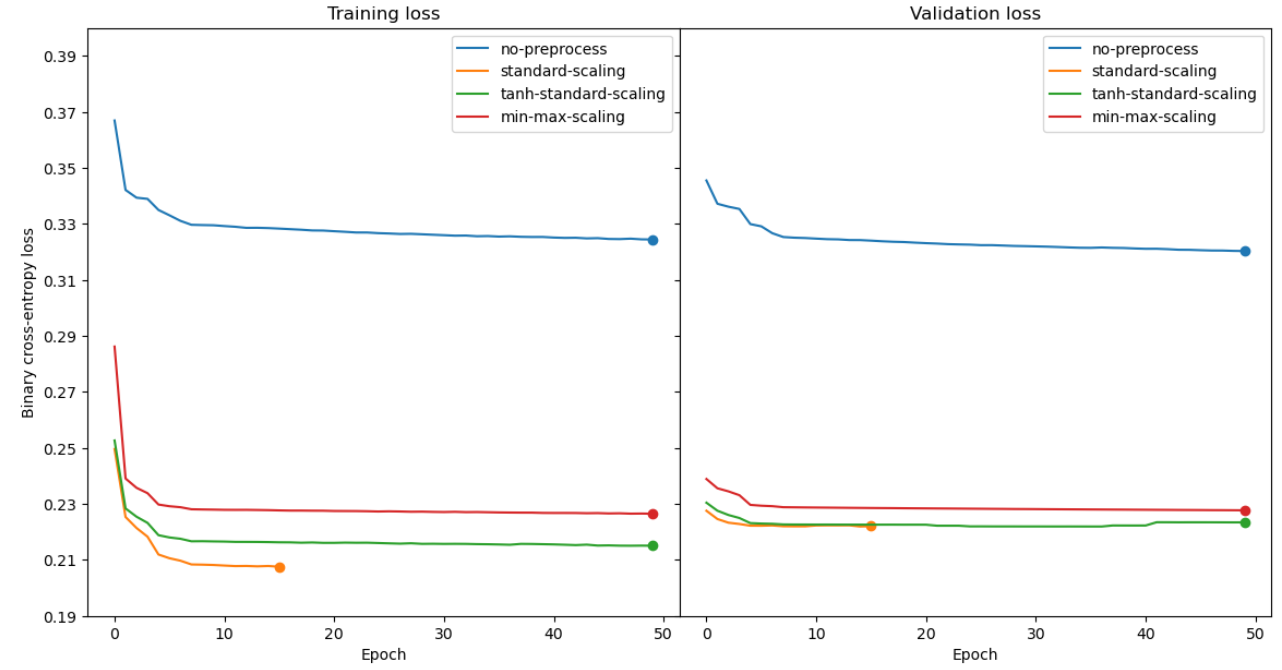
\includegraphics[width=0.975\textwidth]{Figures/loss-cv.png}
\end{center}

% \begin{minipage}{.325\textwidth}
% \captionof{subfigure}{DCSBM: $f_{k,j}(\theta_i)=\theta_i\nu_{k,j}$}
% \vspace*{-.25cm}
% \includegraphics[width=0.975\textwidth]{Pictures/dcsbm_sim.pdf}
% \end{minipage}
% \begin{minipage}{.325\textwidth}
% \captionof{subfigure}{Quadratic: $f_{k,j}(\theta_i)=\alpha_{k,j}\theta_i^2+\beta_{k,j}\theta$}
% \vspace*{-.25cm}
% \includegraphics[width=0.975\textwidth]{Pictures/quadratic_sim.pdf}
% \end{minipage}
% \vspace*{-.25cm}
% \captionof{figure}{Scatterplots of the two-dimensional ASE of simulated graphs arising from simple models, and true underlying latent curves (in black). For each graph, $n=1000$ with $K=2$ communities of equal size. For {(a)} and {(b)}, $\bm\nu_1=[3/4,1/4]$, $\bm\nu_2=[1/4,3/4]$ and $\theta_i\sim\text{Beta}(1,1)$. For {(c)}, $\bm\alpha_k=[-1, -4]$, $\bm\beta_k=[1,1]$, $\bm\gamma_k=[0,0]$ and $\theta_i\sim\text{Beta}(2,1)$.}
% %\label{sim_graphs}
% \vspace*{.25cm}
% \centering
\begin{tabular}{c | c}
\toprule
Dataset & Validation accuracy  \\
\midrule
Synthetic data with non-normal distributions & 95.65\%  \\
Synthetic data with uniform distributions & 98.65\% \\
\bottomrule 
\end{tabular}
% \vspace*{-.1cm}
% \captionof{table}{ARI for communities estimated using LSBM and alternative methodologies on the embeddings in Figure~1.}
%
% \end{center}
}

%%%%%%%%%%%%%%%%%%%%%%%%%%%%%%%%%%%%%%%%%%%%%%%%%%%%%%%%%%%%%%%%%%%%%%%%%%%%%%
% \headerbox{4. Posterior inference}{name=constrained,column=2,span=1,row=1, below=meg, above=picture}{
%   %%%%%%%%%%%%%%%%%%%%%%%%%%%%%%%%%%%%%%%%%%%%%%%%%%%%%%%%%%%%%%%%%%%%%%%%%%%%%%
%
% \begin{itemize}[leftmargin=.15in]
% \item After marginalisation of $(f_{k,j},\sigma^2_{k,j})$ and $\bm\eta$, inference is limited to the community allocations $\vec z$ and parameters $\bm\theta$. 
% \item The posterior distribution $p(\vec z,\bm\theta,K\mid\hat{\mvec X})$ is analytically intractable; inference is performed using \icl{MCMC methods}. 
% %\item Possible moves: 
% \begin{itemize}
% \item Resample the community allocations $\vec z$;
% \item Resample the latent parameters $\vec\theta$;
% \item Split-merge communities;
% \item Add or remove an empty community;
% \item \textit{If prior on kernels is used}: resample kernels. 
% \end{itemize}
% \item The kernel function is usually assumed to be in inner product form, with Zellner’s $g$-prior on the scaling matrix. 
% \end{itemize}
% }

%%%%%%%%%%%%%%%%%%%%%%%%%%%%%%%%%%%%%%%%%%%%%%%%%%%%%%%%%%%%%%%%%%%%%%%%%%%%%%
%\headerbox{4. Background: network models}{name=pmf,column=2,span=1,row=0, above=meg}{
  %%%%%%%%%%%%%%%%%%%%%%%%%%%%%%%%%%%%%%%%%%%%%%%%%%%%%%%%%%%%%%%%%%%%%%%%%%%%%%

%\noindent 
%Considering only the point process marks $(x_1,y_1),(x_2,y_2),\dots,(x_m,y_m)$, it is possible to construct the \icl{edge set} $E$. The pair $(x,y)$ belongs to $E$ only if \icl{at least one connection} from $x$ to $y$ is observed. From $E$, the corresponding \icl{adjacency matrix} $\vecc A$ is obtained:
%\begin{equation}
%A_{ij}=\left\{\begin{array}{ll} 1 & \text{if}\ (i,j)\in E, \\ 0 & \text{otherwise.} \end{array}\right. 
%\end{equation}
%\noindent A successful approach for prediction of \icl{new positive entries} in the adjacency matrix is based on \icl{latent feature models (LFM)} [2]. The probability of a connection between two nodes $x$ and $y$ is expressed as a function of node-specific $d$-dimensional latent features $\vec a_x$ and $\vec b_y$: 
%$\mathbb P(A_{ij}=1)=f(\vec a_i,\vec b_j)$.
%\fbox{\parbox{.97\textwidth}{\icl{Main issue:} LFMs are only suitable for matrices, not for point process data.}} 
%}

%%%%%%%%%%%%%%%%%%%%%%%%%%%%%%%%%%%%%%%%%%%%%%%%%%%%%%%%%%%%%%%%%%%%%%%%%%%%%%
  \headerbox{7. Automating the  preprocessing step}{name=results,column=2,span=3,below=picture}{
%%%%%%%%%%%%%%%%%%%%%%%%%%%%%%%%%%%%%%%%%%%%%%%%%%%%%%%%%%%%%%%%%%%%%%%%%%%%%%

\noindent
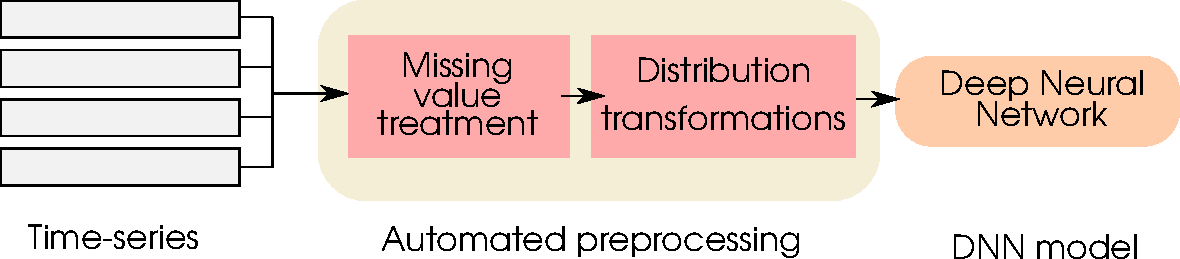
\includegraphics[width=\textwidth]{Figures/automated-preprocessing-diagram.pdf} 

\noindent
TODO: explain diagram
Mention selection informed by either heuristics or learned as part of backpropagation.

% \begin{center}
% \begin{minipage}{.325\textwidth}
% \centering
% \captionof{subfigure}{Harry Potter enmity graph}
% \vspace*{-.25cm}
% \includegraphics[width=\textwidth]{Pictures/x12_harry.pdf} 
% \end{minipage}
% \begin{minipage}{.325\textwidth}
% \centering
% \captionof{subfigure}{\textit{Drosophila} connectome} 
% \vspace*{-.25cm}
% \includegraphics[width=\textwidth]{Pictures/ddroso_12.pdf} 
% \end{minipage}
% \begin{minipage}{.325\textwidth}
% \centering
% \captionof{subfigure}{ICL computer laboratories network}
% \vspace*{-.25cm}
% \includegraphics[width=\textwidth]{Pictures/icl2_12.pdf} 
% \end{minipage}
% \vspace*{-.25cm}
% \captionof{figure}{Two-dimensional embeddings, estimated communities and true labels for three real-world dataset.}
%
% \vspace*{.25cm}
% \centering
% \begin{tabular}{c | cccccccc}
% \toprule
% Method & LSBM$(\hat{\mvec X})$ & GMM$(\hat{\mvec X})$ & GMM$(\tilde{\mvec X})$ & SCSC$(\hat{\mvec X})$ & PGP$(\hat{\mvec X})$ & HLouvain & HClust$(\hat{\mvec X})$ \\
% \midrule
% \textit{Drosophila} connectome & 0.875 & 0.599 & 0.585 & 0.667 & 0.555 & 0.087 & 0.321 \\
% ICL computer laboratories & 0.940 & 0.659 & 0.766 & 0.921 & 0.895 & 0.602 & 0.139 \\
% \bottomrule 
% \end{tabular}
% \vspace*{-.1cm}
% \captionof{table}{ARI for communities estimated using LSBM and alternative methodologies on the \textit{Drosophila} and ICL laboratories networks.}
%
% \end{center}
}

%%%%%%%%%%%%%%%%%%%%%%%%%%%%%%%%%%%%%%%%%%%%%%%%%%%%%%%%%%%%%%%%%%%%%%%%%%%%%%

\headerbox{References}{name=conclusion,column=2,span=3,above=bottom, below=results}{
%\begin{itemize}[leftmargin=.15in] 
%\item \icl{\underline{Latent structure blockmodels}}
%\begin{itemize}[leftmargin=.1cm] 
%\item A model for graphs with group-specific manifold structure;
%\item Gaussian process priors on the unknown latent functions;
%\item Common clustering models are special cases of LSBMs.
%\end{itemize}
%\end{itemize}
{\footnotesize{
\begin{itemize}[leftmargin=.1in] 
\item TODO
% \item Athreya, A. et al. (2018). “Statistical Inference on Random Dot Product Graphs: a Survey”. Journal of Machine Learning Research 18, 1--92.
% \item Athreya, A. et al. (2021). “On Estimation and Inference in Latent Structure Random Graphs”. Statistical Science 36.1, 68--88.
% \item Hoff, P. D. et al. (2002). “Latent space approaches to social network analysis”. Journal of the American Statistical Association 97, 1090--1098. 
% %\item Holland, P. W., K. B. Laskey, and S. Leinhardt (1983). “Stochastic blockmodels: First steps”. Social Networks 5.2, 109--137.
% %\item Karrer, B. and M. E. J. Newman (2011). “Stochastic blockmodels and community structure in networks”. Physical Review E 83 (1).
% \item Rubin-Delanchy, P. (2020). “Manifold structure in graph embeddings”. Advances in Neural Information Processing Systems 33, %Ed. by H. Larochelle et al. Vol. 33. Curran Associates, Inc.,  
% 11687–11699.
\end{itemize}
}}
}

%%%%%%%%%%%%%%%%%%%%%%%%%%%%%%%%%%%%%%%%%%%%%%%%%%%%%%%%%%%%%%%%%%%%%%%%%%%%%%
% \headerbox{Paper and \textit{python} library \texttt{lsbm}}{name=future,column=2,above=bottom, below=results}{
% \centering
% \begin{minipage}{0.49\textwidth}
% \centering
% \icl{Paper} \\
% \noindent\includegraphics[width=0.575\textwidth]{Pictures/qr_paper.png}
% \end{minipage}
% \begin{minipage}{0.49\textwidth}
% \centering
% \icl{\textit{python} library \texttt{lsbm}} \\
% \includegraphics[width=0.575\textwidth]{Pictures/qr_git.png}
% \end{minipage}
% %{\footnotesize
% %\noindent{
% %\begin{itemize}[leftmargin=.15in] 
% %\item[[1\hspace{-.5em}]] Price-Williams, M. and Heard, N. A. (2019). “Nonparametric self-exciting models for computer network traffic”. In: Statistics and Computing 30,  209-220. 
% %\item[[2\hspace{-.5em}]] Hoff, P. D., Raftery, A. E., and Handcock, M. S. (2002). “Latent space approaches to social network analysis”. In: Journal of the American Statistical Association 97(460),  1090-1098.
% %\item[[3\hspace{-.5em}]] Sanna Passino, F., Turcotte, M. J. M., and Heard, N. A. (2020). “Graph link prediction in computer networks using Poisson matrix factorisation”. In: arXiv e-prints. arXiv: 2001.09456.
% %\item[[4\hspace{-.5em}]] Kingma, D. P. and Ba, J. (2015) Adam: a method for stochastic optimization. In 3rd International Conference on Learning Representations, ICLR (eds. Y. Bengio and Y. LeCun).
% %\end{itemize} %\\[0.2cm]
% %}}
% }

\end{poster}

\end{document}

